\documentclass[tikz,border=10pt]{standalone}
% No extra TikZ libraries are needed for this figure.
\begin{document}
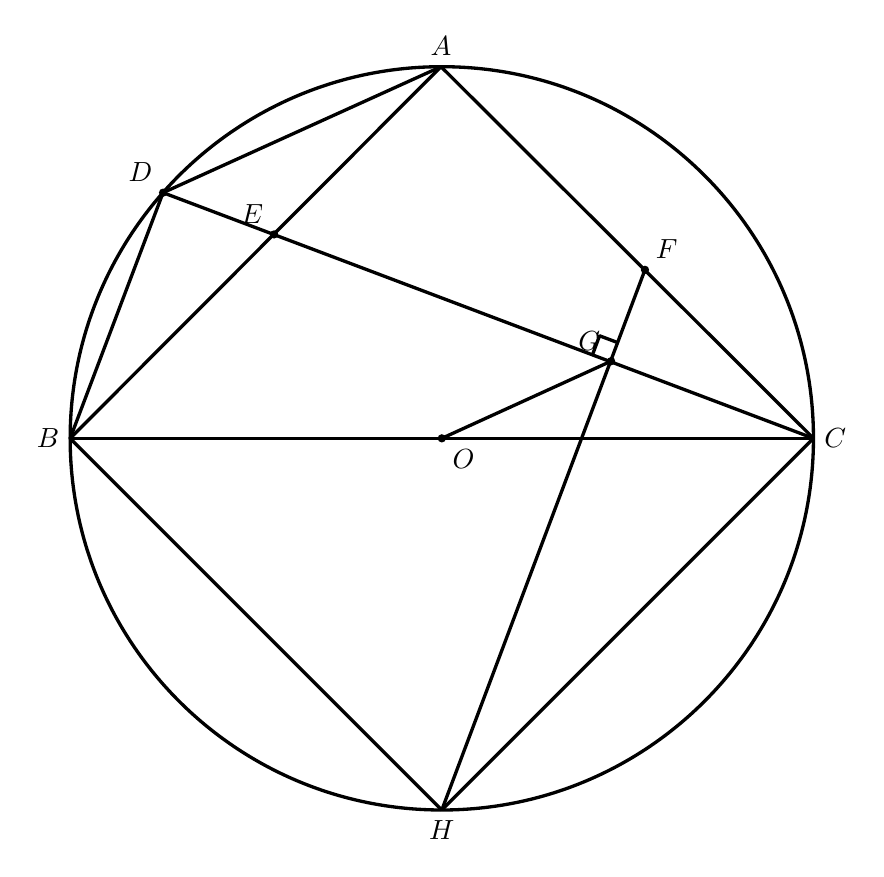
\begin{tikzpicture}[line width=1.2pt, line join=round]
  % Coordinates: 1 unit = 100 px, origin at O, y flipped
  \coordinate (O) at (0,0);
  \coordinate (A) at (-0.01,4.72);
  \coordinate (B) at (-4.72,0);
  \coordinate (C) at (4.72,0);
  \coordinate (D) at (-3.54,3.12);
  \coordinate (E) at (-2.13,2.59);
  \coordinate (F) at (2.58,2.14);
  \coordinate (G) at (2.15,0.98);
  \coordinate (H) at (0,-4.72);

  % Circle with centre O
  \draw (O) circle (4.72);

  % Segments
  \draw (B) -- (C);   % diameter BC
  \draw (A) -- (C);   % AC through F
  \draw (B) -- (A);   % BA through E
  \draw (D) -- (C);   % DC through E and G
  \draw (F) -- (H);   % FH through G
  \draw (O) -- (G);   % OG
  \draw (B) -- (H);
  \draw (C) -- (H);
  \draw (B) -- (D);
  \draw (A) -- (D);

  % Right-angle mark at G between GF and GD
  \draw (2.237,1.215) -- (2.003,1.3025) -- (1.916,1.068);

  % Small dots at E, F, G, O, D
  \foreach \p in {D,E,F,G,O} \fill (\p) circle (1.5pt);

  % Labels
  \node[above] at (A) {$A$};
  \node[left]  at (B) {$B$};
  \node[right] at (C) {$C$};
  \node[above left] at (D) {$D$};
  \node[above left] at (E) {$E$};
  \node[above right] at (F) {$F$};
  \node[above left] at (G) {$G$};
  \node[below] at (H) {$H$};
  \node[below right] at (O) {$O$};
\end{tikzpicture}
\end{document}